\documentclass[hide notes,intlimits]{beamer}

\mode<presentation>
{
  \usetheme[footline]{PISMshade}
  \setbeamercovered{transparent}
}

% load packages
\usepackage{multimedia}
\usepackage[english]{babel}
\usepackage[latin1]{inputenc}
\usepackage[T1]{fontenc}
\usepackage{lmodern}
\usepackage{pdfpages}
\usepackage[multidot]{grffile}

%\setbeameroption{show notes on second screen=right}

\usepackage{tikz}
\usetikzlibrary{shapes,arrows}
\usetikzlibrary{shadows}

\definecolor{dark red}{HTML}{E41A1C}
\definecolor{dark green}{HTML}{4DAF4A}
\definecolor{dark violet}{HTML}{984EA3}
\definecolor{dark blue}{HTML}{084594}
\definecolor{dark orange}{HTML}{FF7F00}
\definecolor{light blue}{HTML}{377EB8}
\definecolor{light red}{HTML}{FB9A99}
\definecolor{light violet}{HTML}{CAB2D6}

\setbeamercolor{boxed}{fg=black,bg=light blue!25}
\graphicspath{{figures/}}

% Define block styles
\tikzstyle{initialization} = [ellipse, draw, 
    text badly centered, draw=dark violet,
        % The filling: 
        top color=white, 
        bottom color=dark violet]
\tikzstyle{initialization faded} = [ellipse, draw, 
    text badly centered, draw=dark violet!50,
        % The filling: 
        top color=white, 
        bottom color=dark violet!25]
\tikzstyle{hindcast} = [ellipse, draw,
    text badly centered, rounded corners,draw=dark orange,
        % The filling: 
        top color=white, 
        bottom color=dark orange]
\tikzstyle{hindcast faded} = [ellipse, draw,
    text badly centered, rounded corners,draw=dark orange!50,
        % The filling: 
        top color=white, 
        bottom color=dark orange!25]
\tikzstyle{forecast} = [ellipse, draw,
    text badly centered, rounded corners,draw=dark blue,
        % The filling: 
        top color=white, 
        bottom color=dark blue]
\tikzstyle{forecast faded} = [ellipse, draw,
    text badly centered, rounded corners,draw=dark blue!50,
        % The filling: 
        top color=white, 
        bottom color=dark blue!50]
\tikzstyle{arrow line} = [draw, -latex']
\tikzstyle{line} = [draw]

\newenvironment{transbox}[1][]{%
\begin{tikzpicture}
\node[drop shadow,rounded corners,text width=.9\textwidth,fill=white, fill opacity=#1,text opacity=1] \bgroup
}{
\egroup;\end{tikzpicture}} 

\newenvironment{transbox-tight}{%
\begin{tikzpicture}
\node[drop shadow,rounded corners,fill=uaf yellow, fill opacity=0.75,text opacity=1] \bgroup
}{
\egroup;\end{tikzpicture}} 

\newcommand{\jl}{[\![}
\newcommand{\jr}{]\!\hskip 0.003cm ]}
\newcommand{\bpsi}{\boldsymbol{\psi}}
\newcommand{\bPsi}{\boldsymbol{\Psi}}
\newcommand{\bphi}{\boldsymbol{\phi}}
\newcommand{\bPhi}{\boldsymbol{\Phi}}
\newcommand{\bn}{\mathbf{n}}
\newcommand{\bq}{\mathbf{q}}
\newcommand{\bv}{\mathbf{v}}
\newcommand{\D}{\,\mathrm{d}}
\newcommand{\Tsnow}{T_{\text{snow}}}
\newcommand{\Hatm}{H_{\text l}^{\text{atm}}}

\newcommand{\mathtext}[1]{\mathsf{#1}}

% title page
\title[Ice sheet modeling] % (optional, use only with long paper titles)
{The Greenland Ice Sheet}
\subtitle{Will it stay or will it go?}

\author[Aschwanden] % (optional, use only with lots of authors)
{Andy Aschwanden}
% - Give the names in the same order as the appear in the paper.
% - Use the \inst{?} command only if the authors have different
%   affiliation.

% - Use the \inst command only if there are several affiliations.
% - Keep it simple, no one is interested in your street address.

\titlegraphic{\vskip-1.cm\includegraphics[height=4cm]{rcp-final-states-extend}}

\date{}


\subject{The Greenland Ice Sheet}

\begin{document}


\setbeamertemplate{background canvas}
  {
     \tikz{\node[inner sep=0pt,opacity=1.0] {\includegraphics[width=\paperwidth]{uaf_beamer_shade_bg}};}
} 

% insert titlepage
\begin{frame}
  \titlepage
\end{frame}


\setbeamertemplate{background canvas}
  {
} 

\setbeamertemplate{background canvas}
  {
     \tikz{\node[inner sep=0pt,opacity=1] {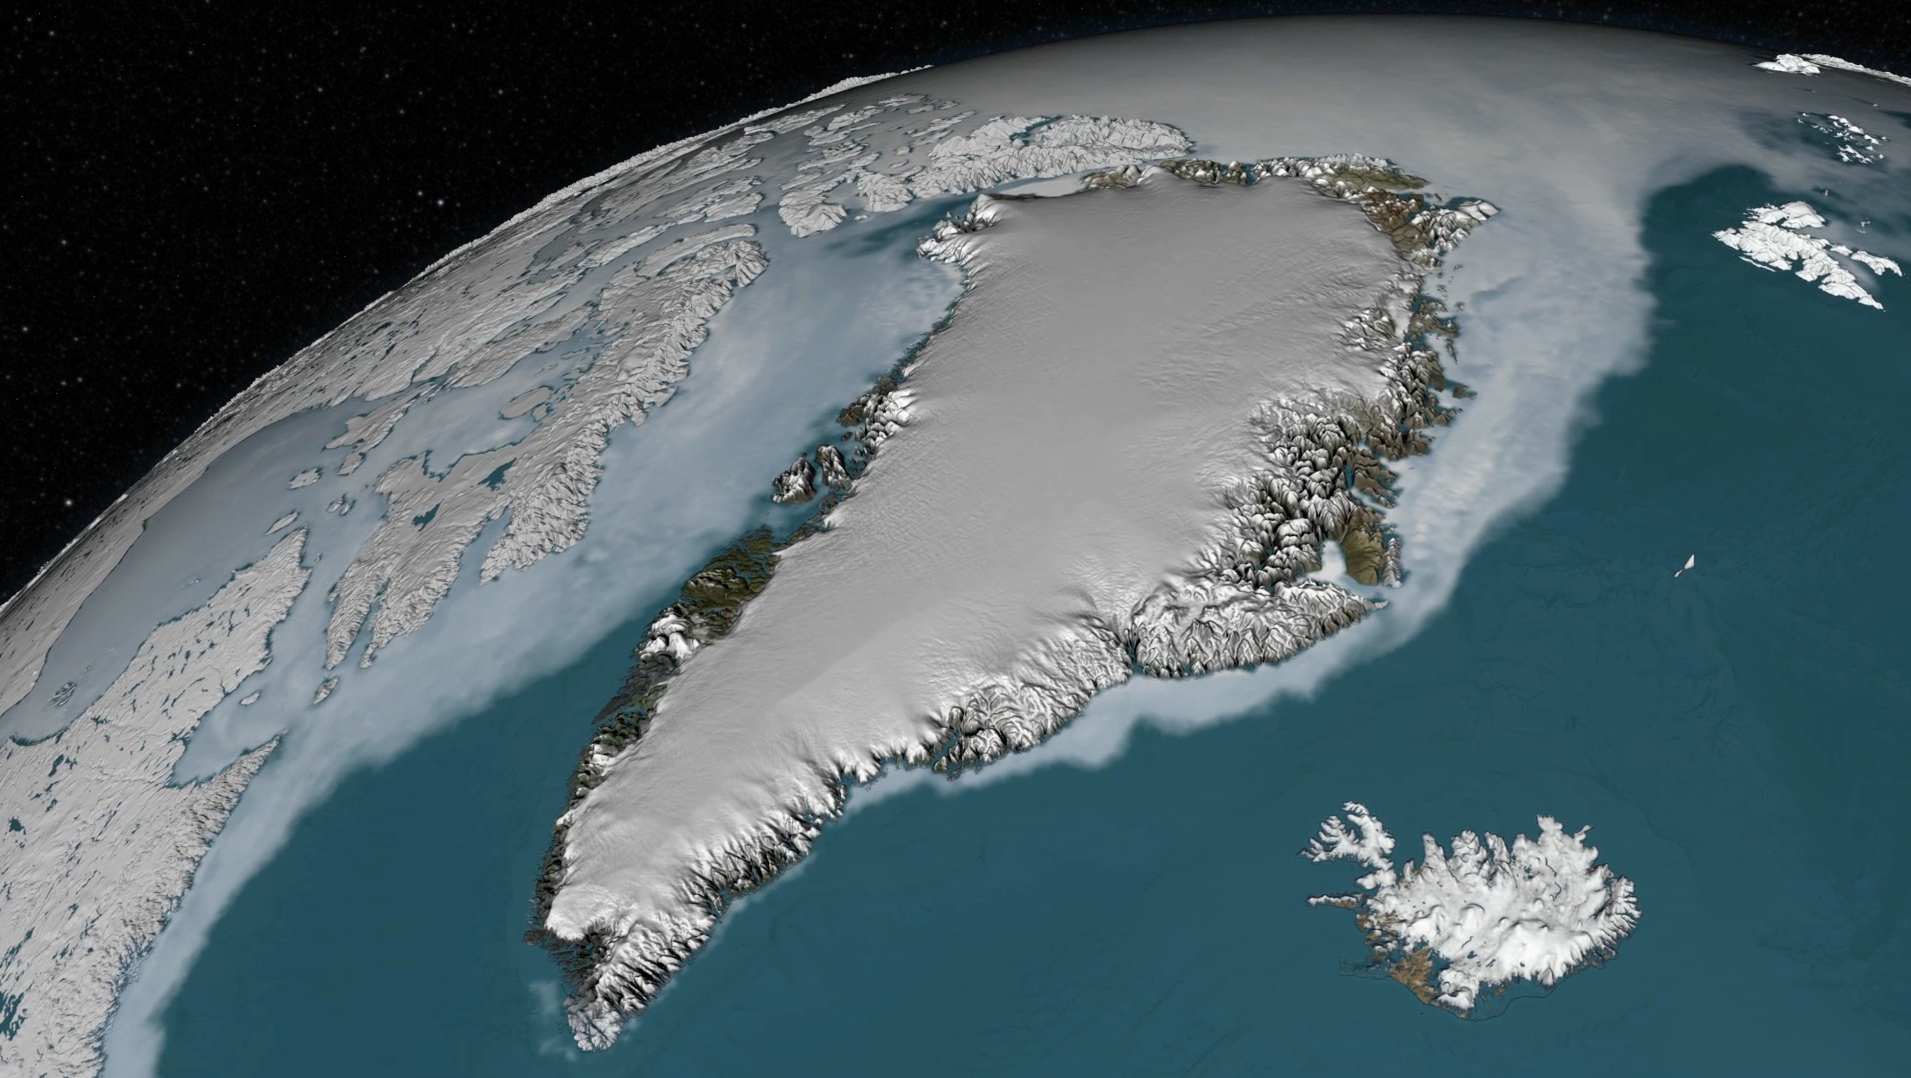
\includegraphics[height=\paperheight,width=\paperwidth]{nasa-mapping-greenland-ice-sheet}};}
} 

\begin{frame}[plain]
\end{frame}

\setbeamertemplate{background canvas}
  {
     \tikz{\node[inner sep=0pt,opacity=.5] {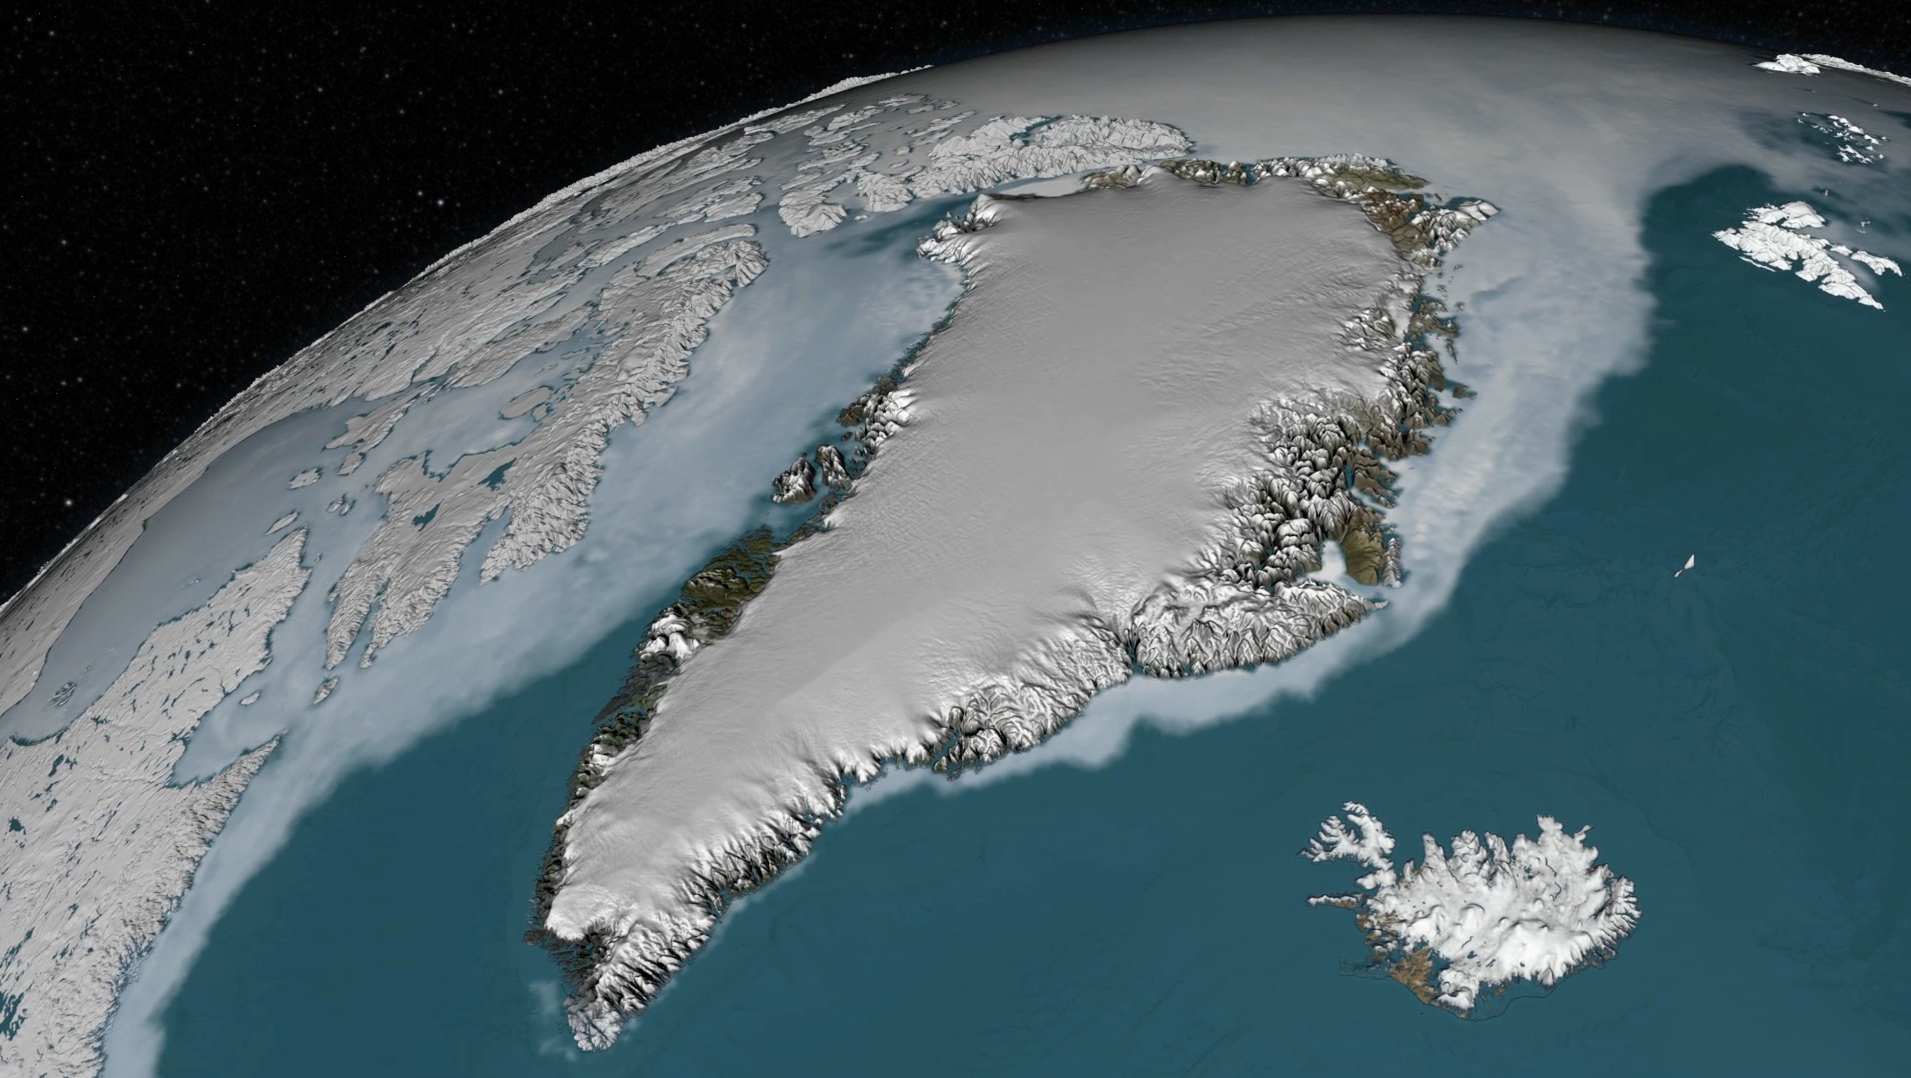
\includegraphics[height=\paperheight,width=\paperwidth]{nasa-mapping-greenland-ice-sheet}};}
} 

\begin{frame}[plain]
    \begin{itemize}
    \item extent of $1200\,\text{km}\,\times 2400\,\text{km}$ \dots it's a ``dwarf continent''
    \item total area: 2.1 million km$^2$
    \item ice covered area:  1.7 million km$^2$
    \item \alert{for comparison: that's 17$\times$ the area of South Korea}
    \item has ice equivalent of 7.2 m of sea-level rise
    \item over past 2 decades: losing mass at an accelerating rate
    \end{itemize}
    \note[item]{Explain why Greenland is of interest}
\end{frame}


\setbeamertemplate{background canvas}
{
%
} 

\begin{frame}[plain]
    \begin{figure}
      \movie[showcontrols=true,loop,width=12cm]{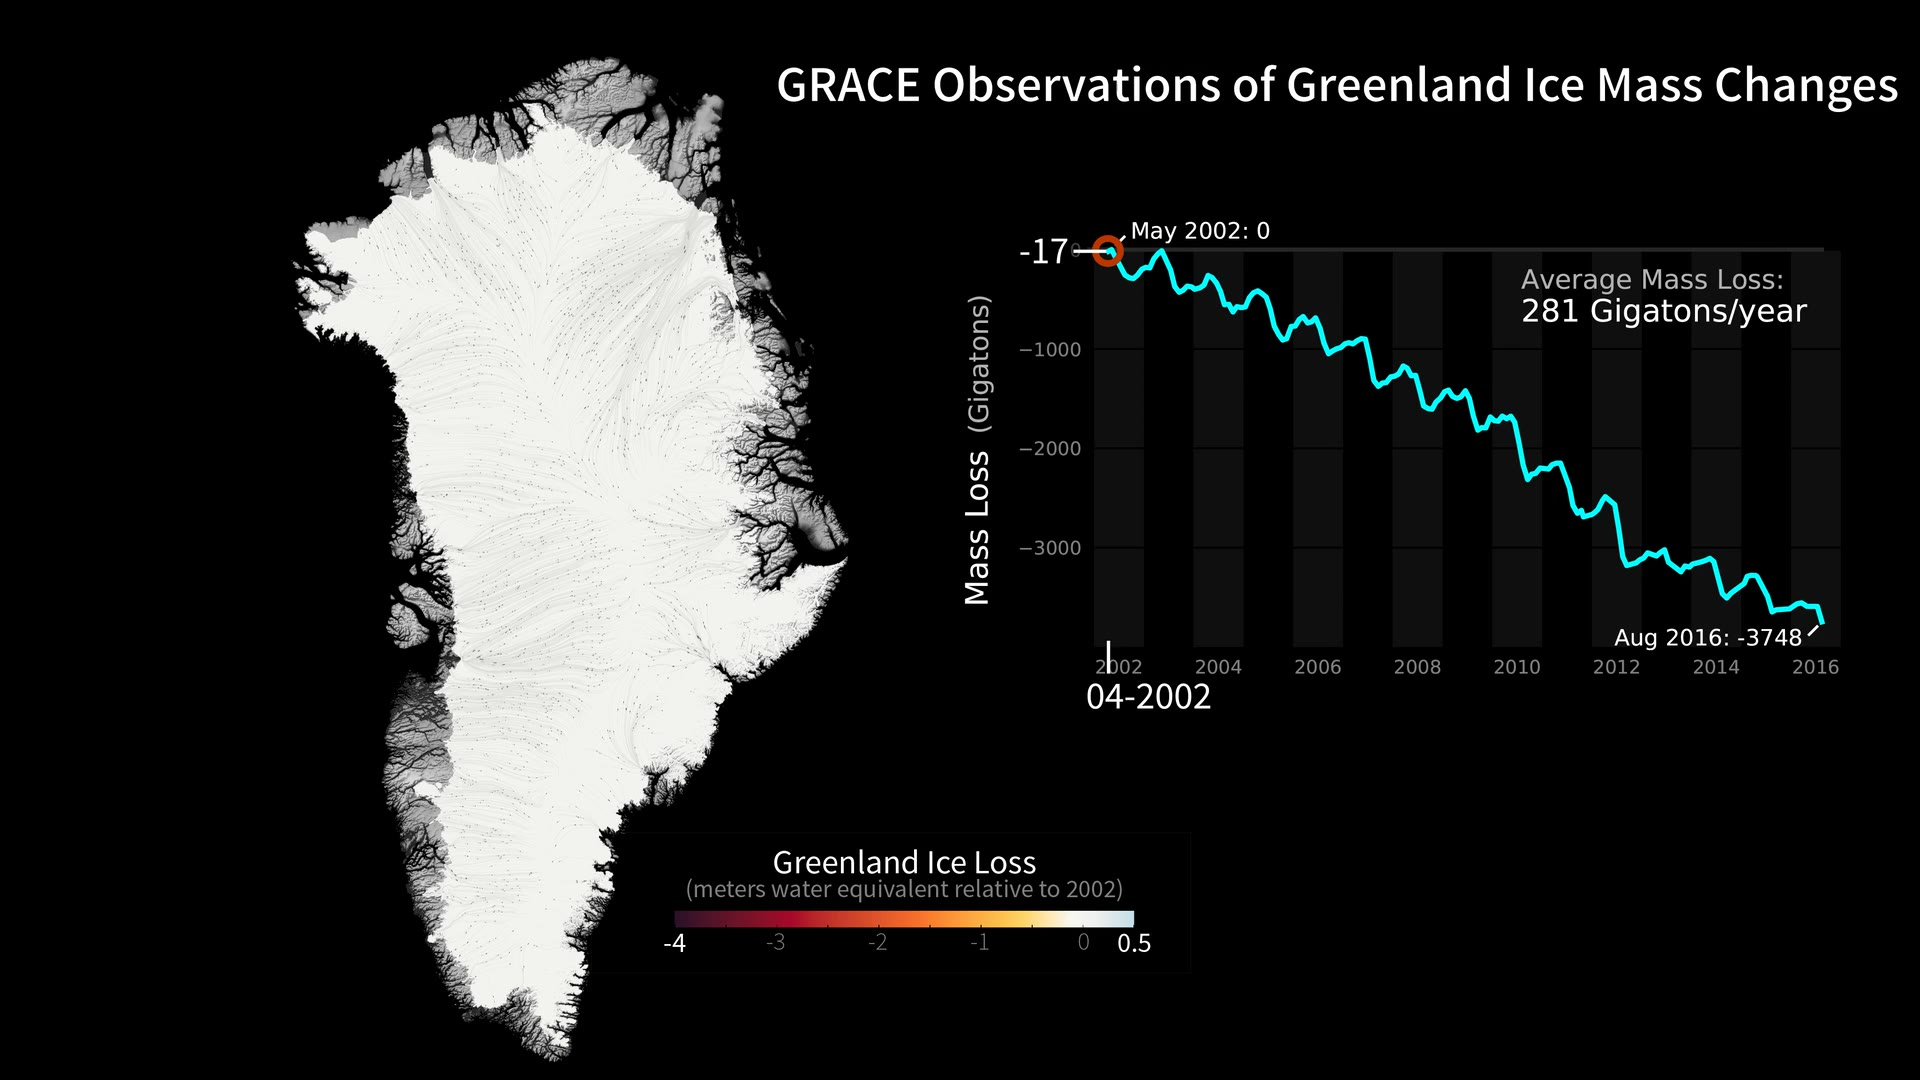
\includegraphics[width=12cm]{../movies/68_grace_greenland_1080p}}{../movies/68_grace_greenland_1080p.mov}
  \end{figure}
  \begin{itemize}
  \item<2> 280\,Gt is about half of Lake Eerie or a 3\,m high layer of water covering South Korea
  \end{itemize}
  \note[item]{show NASA GRACE mass loss animation}
  \note[item]{greatest losses occur on the west coast and SE coast} 
  \note[item]{explain how much 280 Gt really are}
\end{frame}


\begin{frame}
  \frametitle{IPCC AR4, 2007}
  \begin{columns}[c]
    \begin{column}{.4\linewidth}
      \begin{figure}
        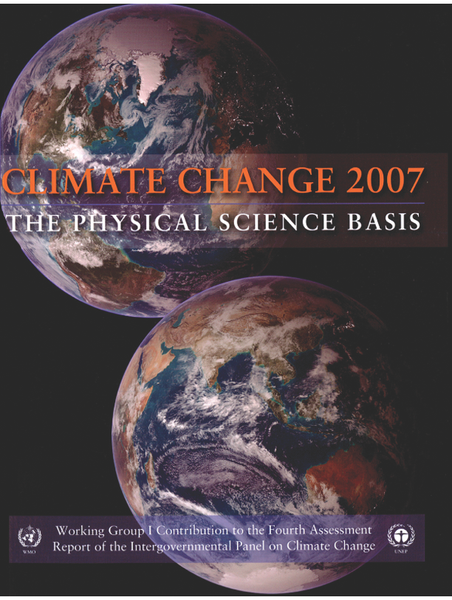
\includegraphics[height=6cm]{ar4-wg1}
      \end{figure}
    \end{column}
    \begin{column}{.5\linewidth}
      \begin{itemize}
      \item No results from ice sheet models included due to the models' inability to track recent changes
      \end{itemize}
    \end{column}
\end{columns}
\end{frame}

\begin{frame}
  \frametitle{IPCC AR5, 2013}
  \begin{columns}[c]
    \begin{column}{.4\linewidth}
      \begin{figure}
        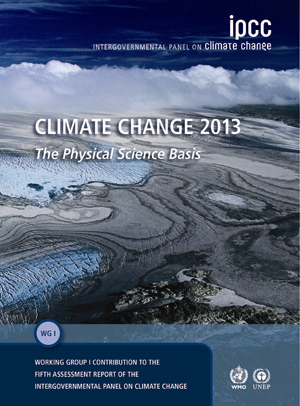
\includegraphics[height=6cm]{ar5-wg1}
      \end{figure}
    \end{column}
    \begin{column}{.6\linewidth}
      \begin{figure}
        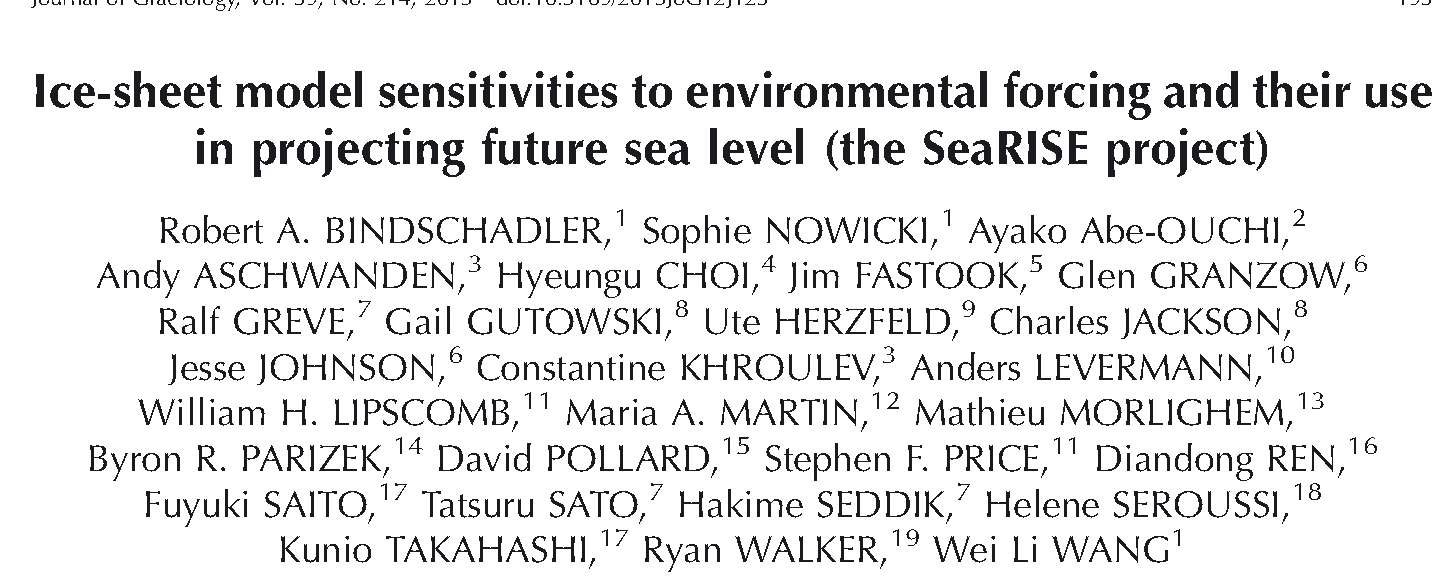
\includegraphics[width=5cm]{searise}
      \end{figure}
      \begin{figure}
        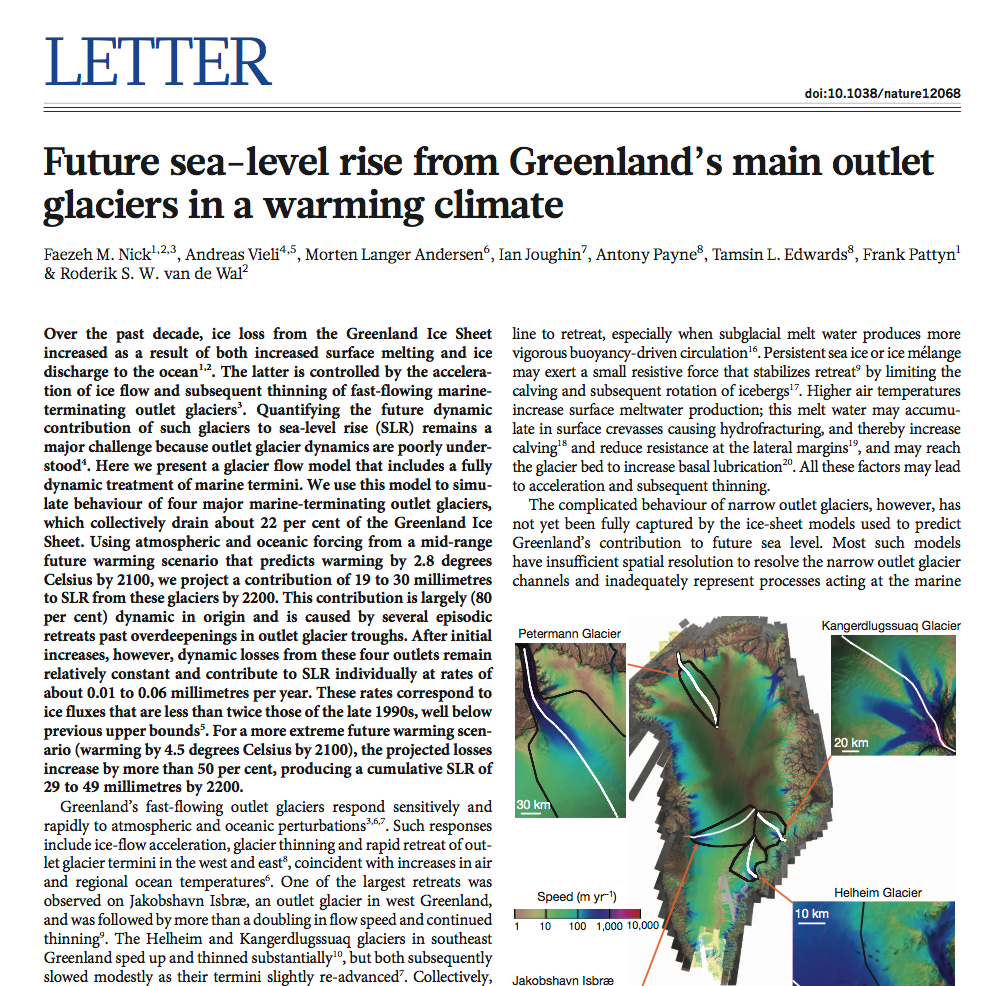
\includegraphics[width=5cm]{nick2013}
      \end{figure}
    \end{column}
  \end{columns}
\end{frame}

\begin{frame}
  \frametitle{Since AR5: Antarctica}
  \begin{columns}[c]
    \begin{column}{.4\linewidth}
      \begin{figure}
        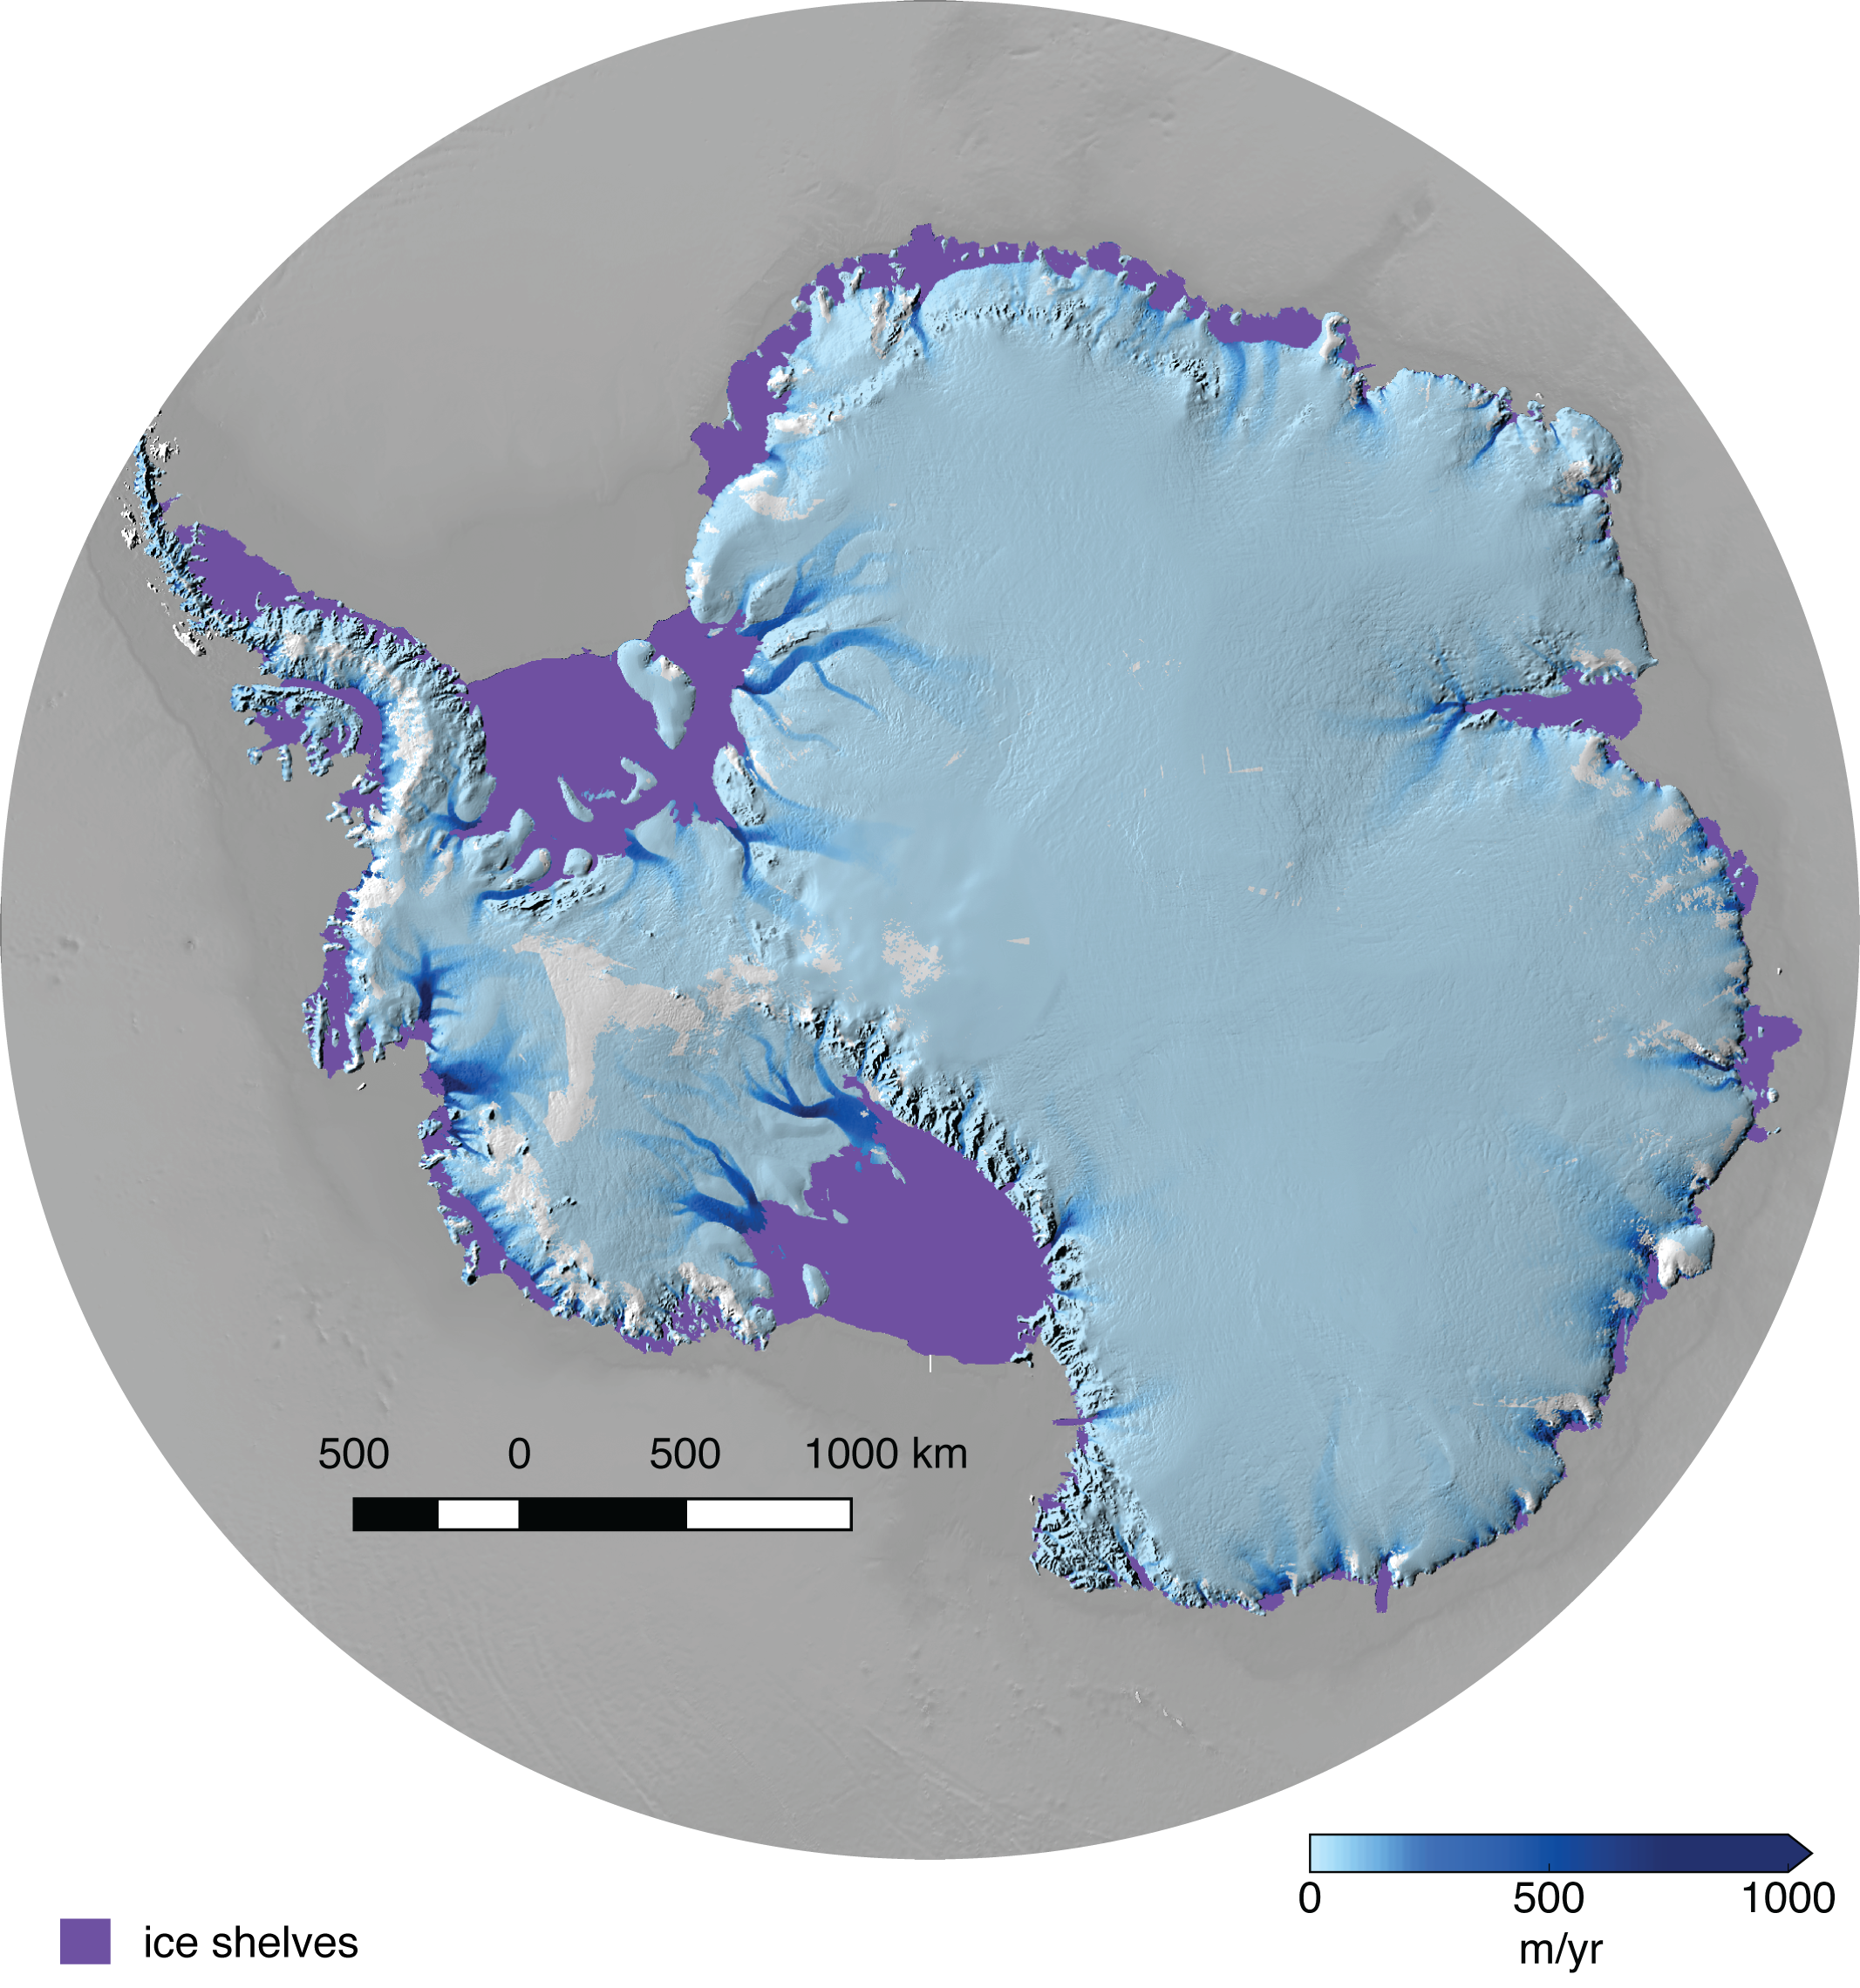
\includegraphics[height=5cm]{ant-shelves}
      \end{figure}
    \end{column}
    \begin{column}{.6\linewidth}
      \begin{figure}
        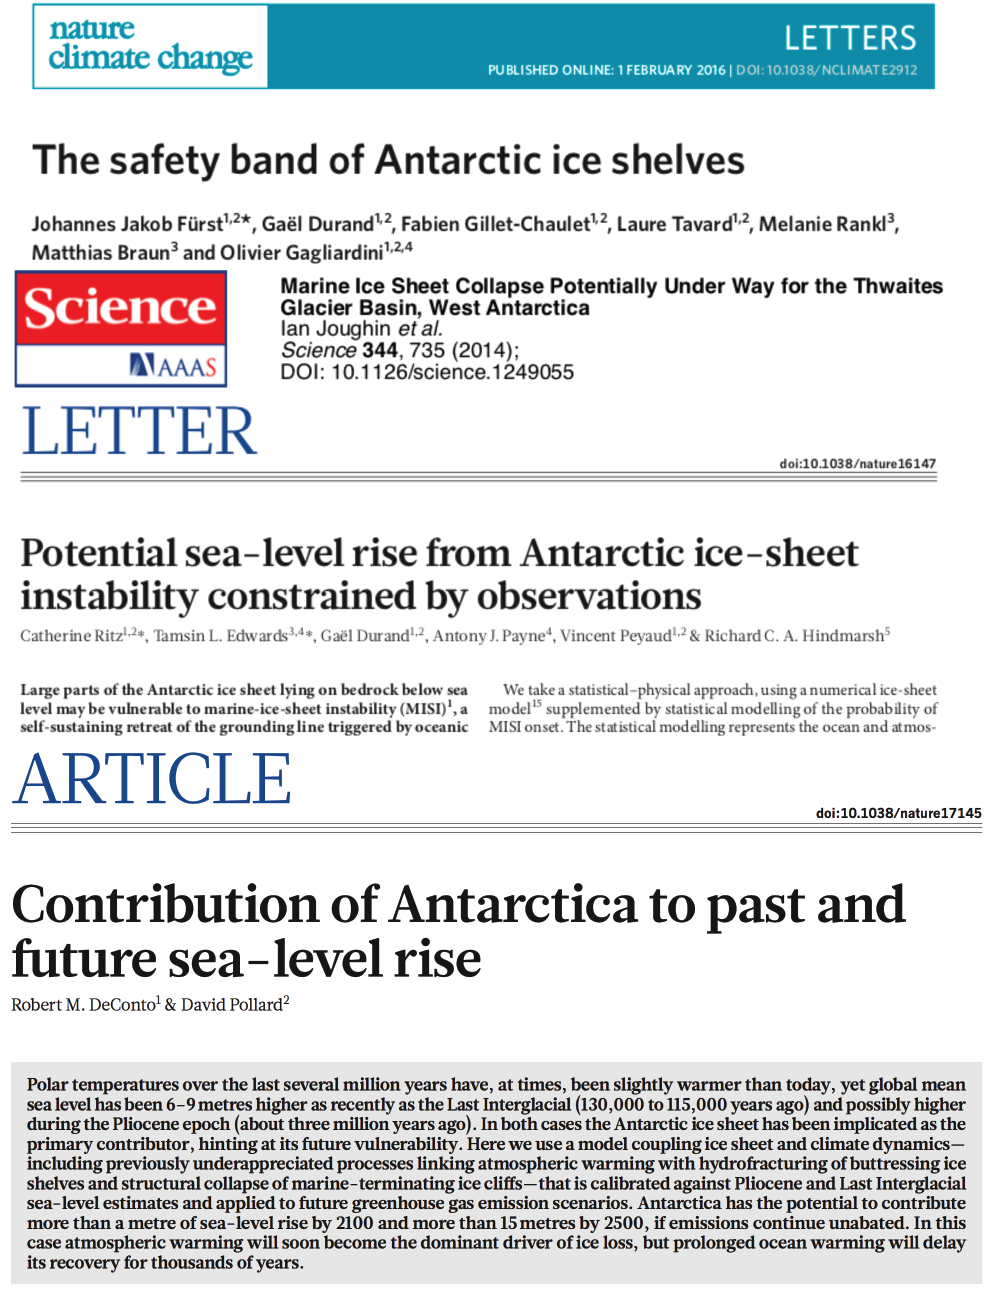
\includegraphics[width=5cm]{recent-ant-pubs}
      \end{figure}
    \end{column}
  \end{columns}
\end{frame}

\begin{frame}
  \frametitle{Since AR5: Greenland}
  \begin{columns}[c]
    \begin{column}{.4\linewidth}
      \begin{figure}
        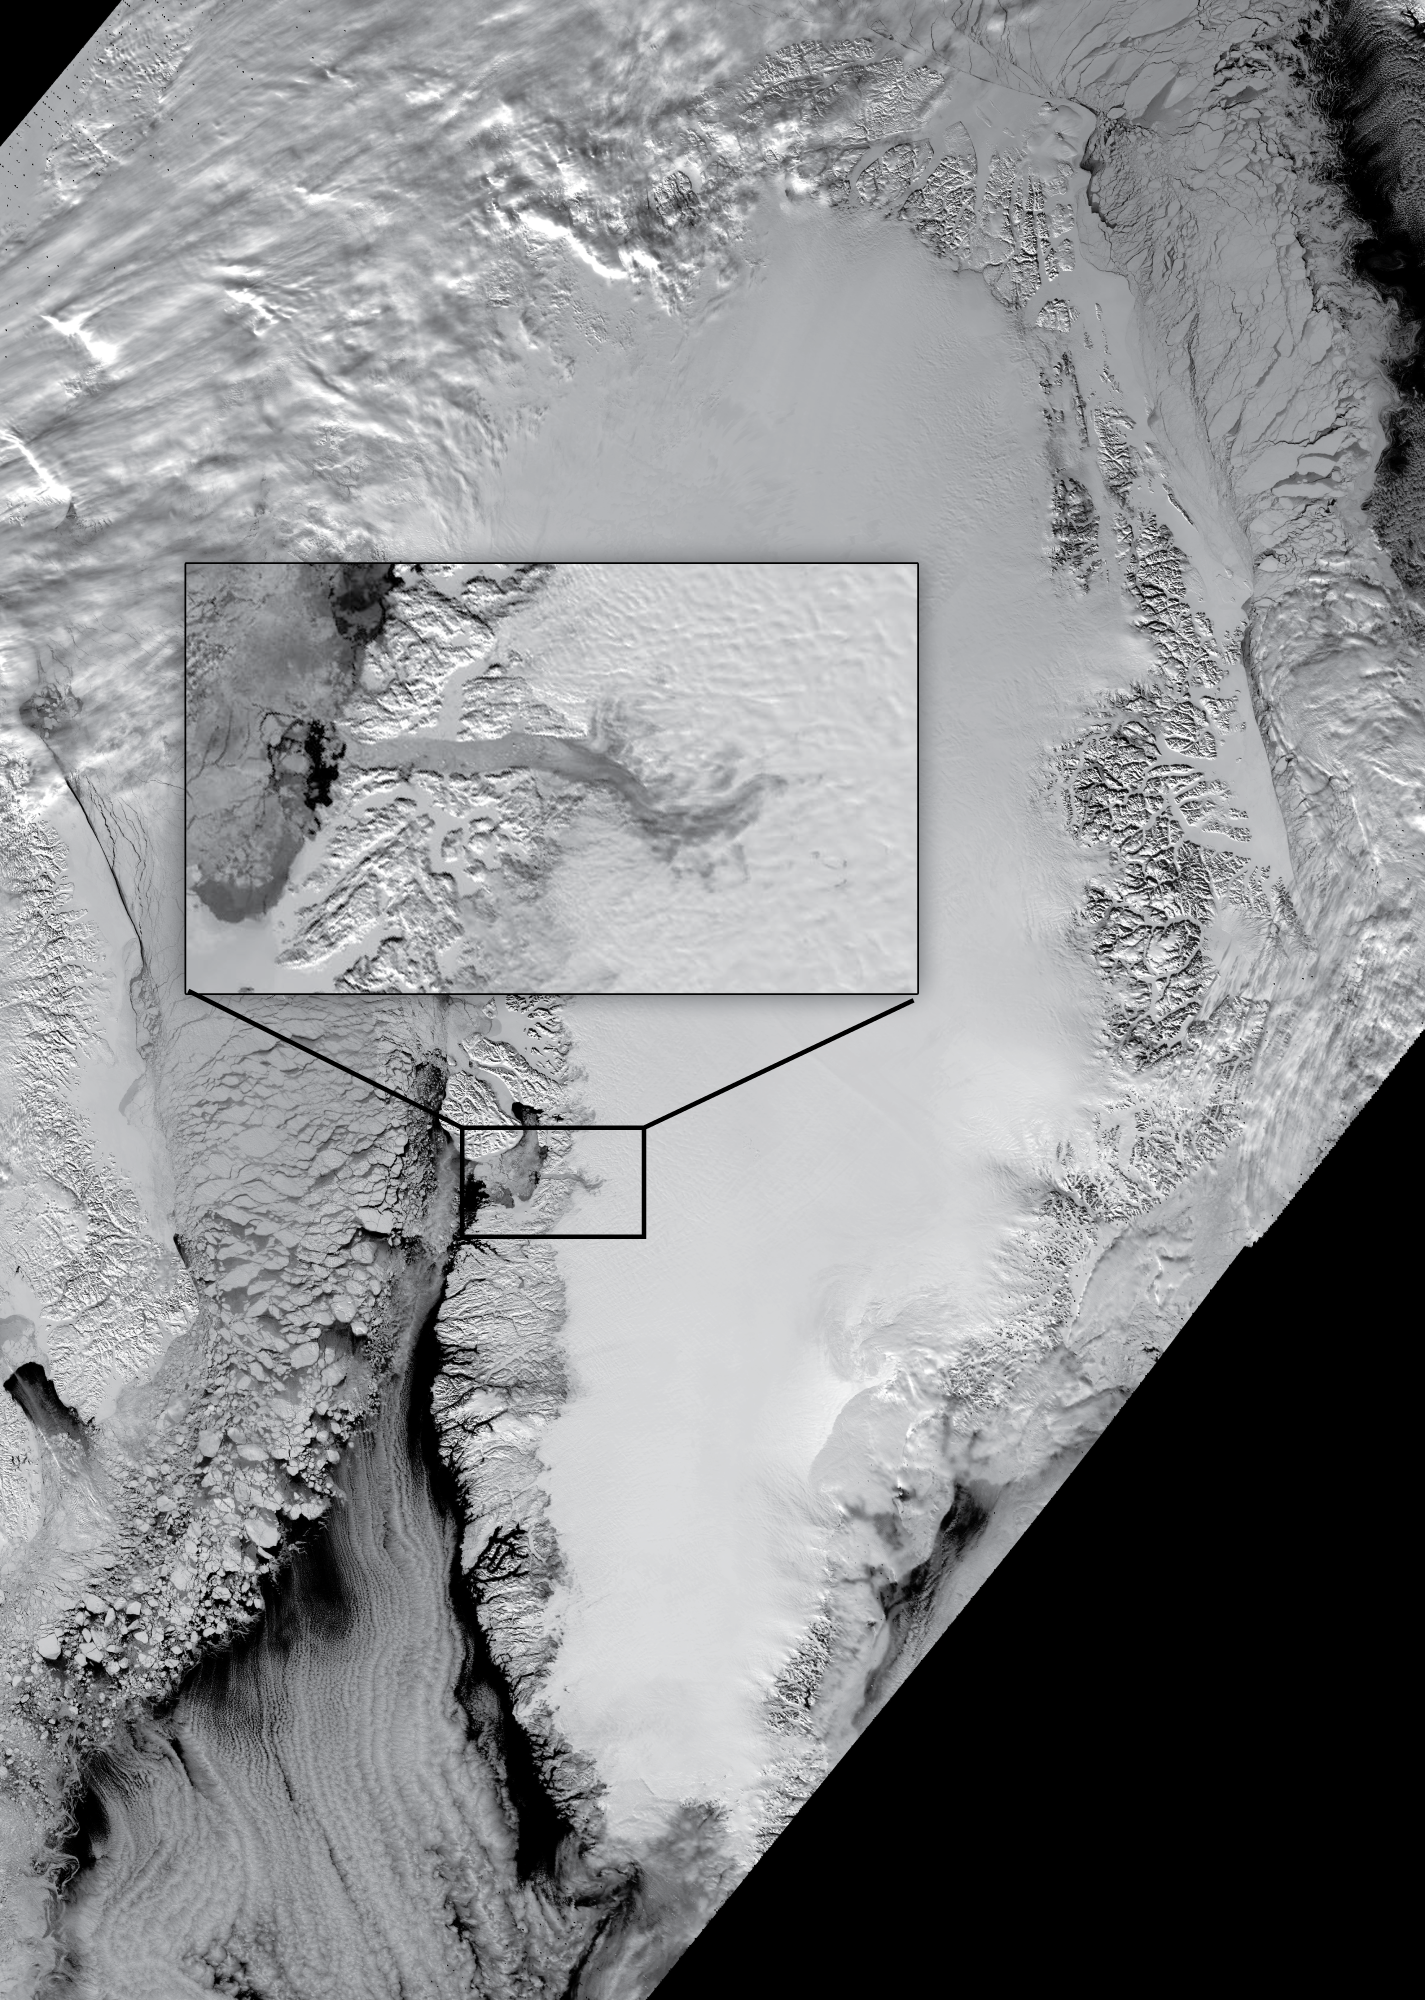
\includegraphics[height=6cm]{MODISGreenlandJakobshavn}
      \end{figure}
    \end{column}
    \begin{column}{.6\linewidth}
      \begin{figure}
        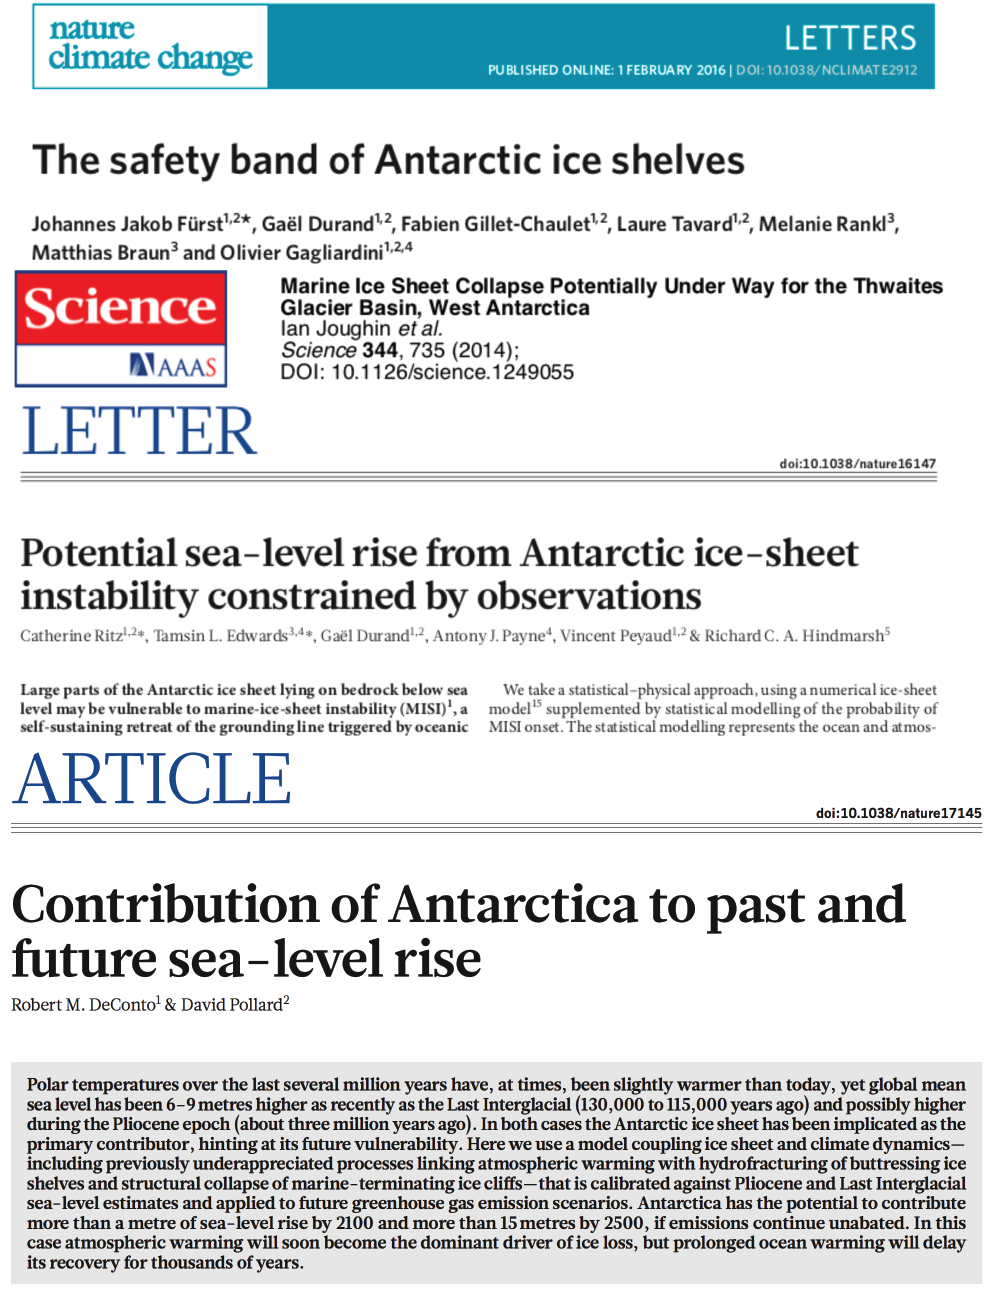
\includegraphics[width=5cm]{recent-ant-pubs}
      \end{figure}
    \end{column}
  \end{columns}
\end{frame}


\begin{frame}{We can capture the present-day flow field}
  \begin{figure}
    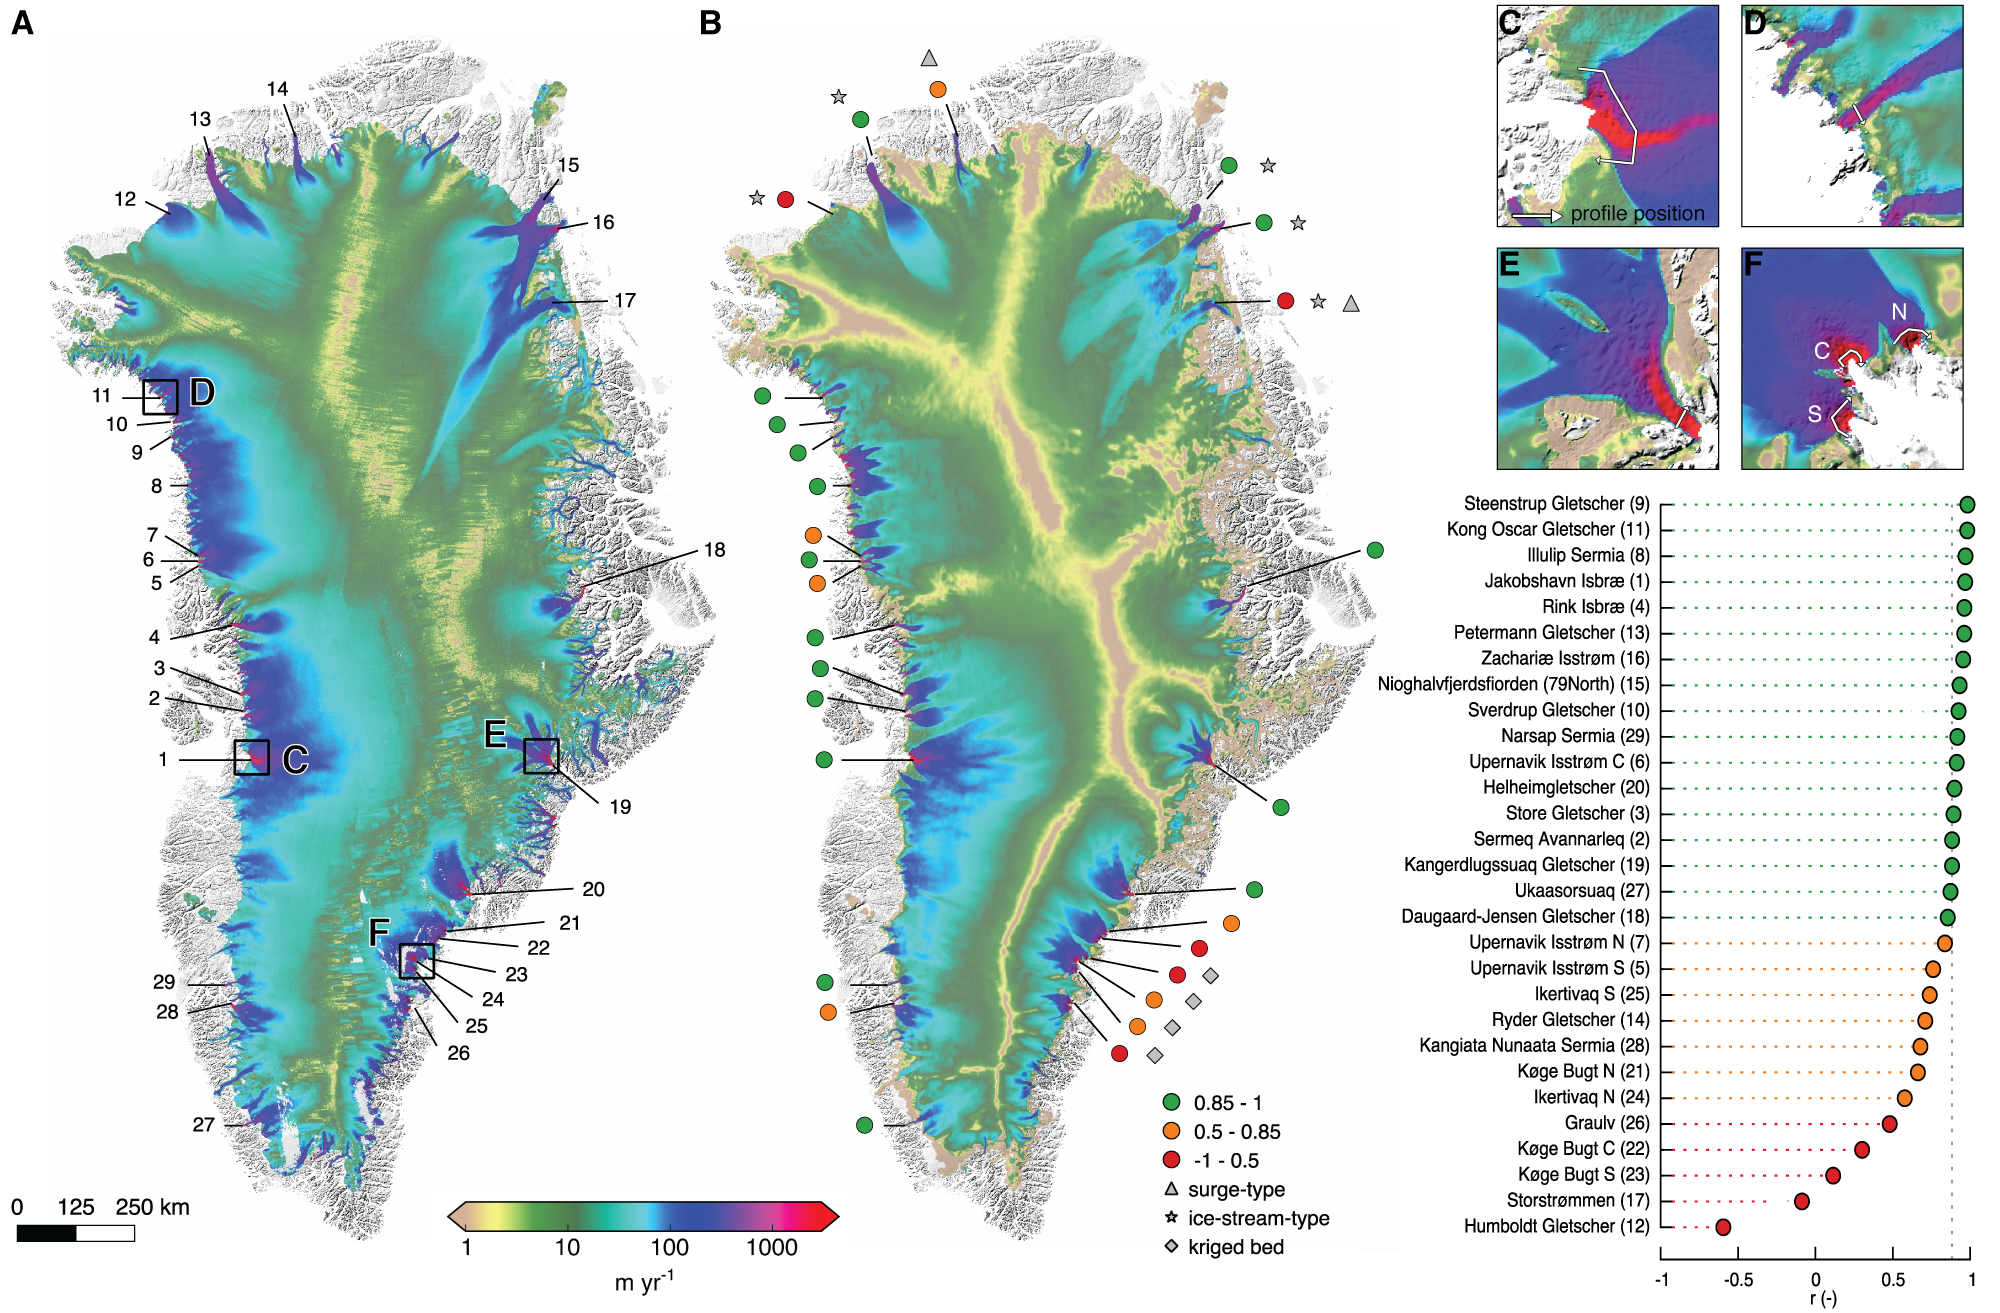
\includegraphics[height=7cm]{greenland-overview-3}
    \\ \scriptsize{Aschwanden, Fahnestock, Truffer (2016) \textit{Nature Communications}}
  \end{figure}
  \note[item]{first time capturing the flow field for the right reason}
  \note[item]{this is quite a break through in ice sheet modeling}
  \note[item]{though not a surprising one}
  \note[item]{it just confirms what students learn in glaciology 100:}
  \note[item]{ice flows downhill}
\end{frame}

\begin{frame}
  \frametitle{Uncertaintiy Analysis}
    \begin{columns}[c]
      \begin{column}{.4\linewidth}
        \vspace{-.25cm}
      \begin{figure}
        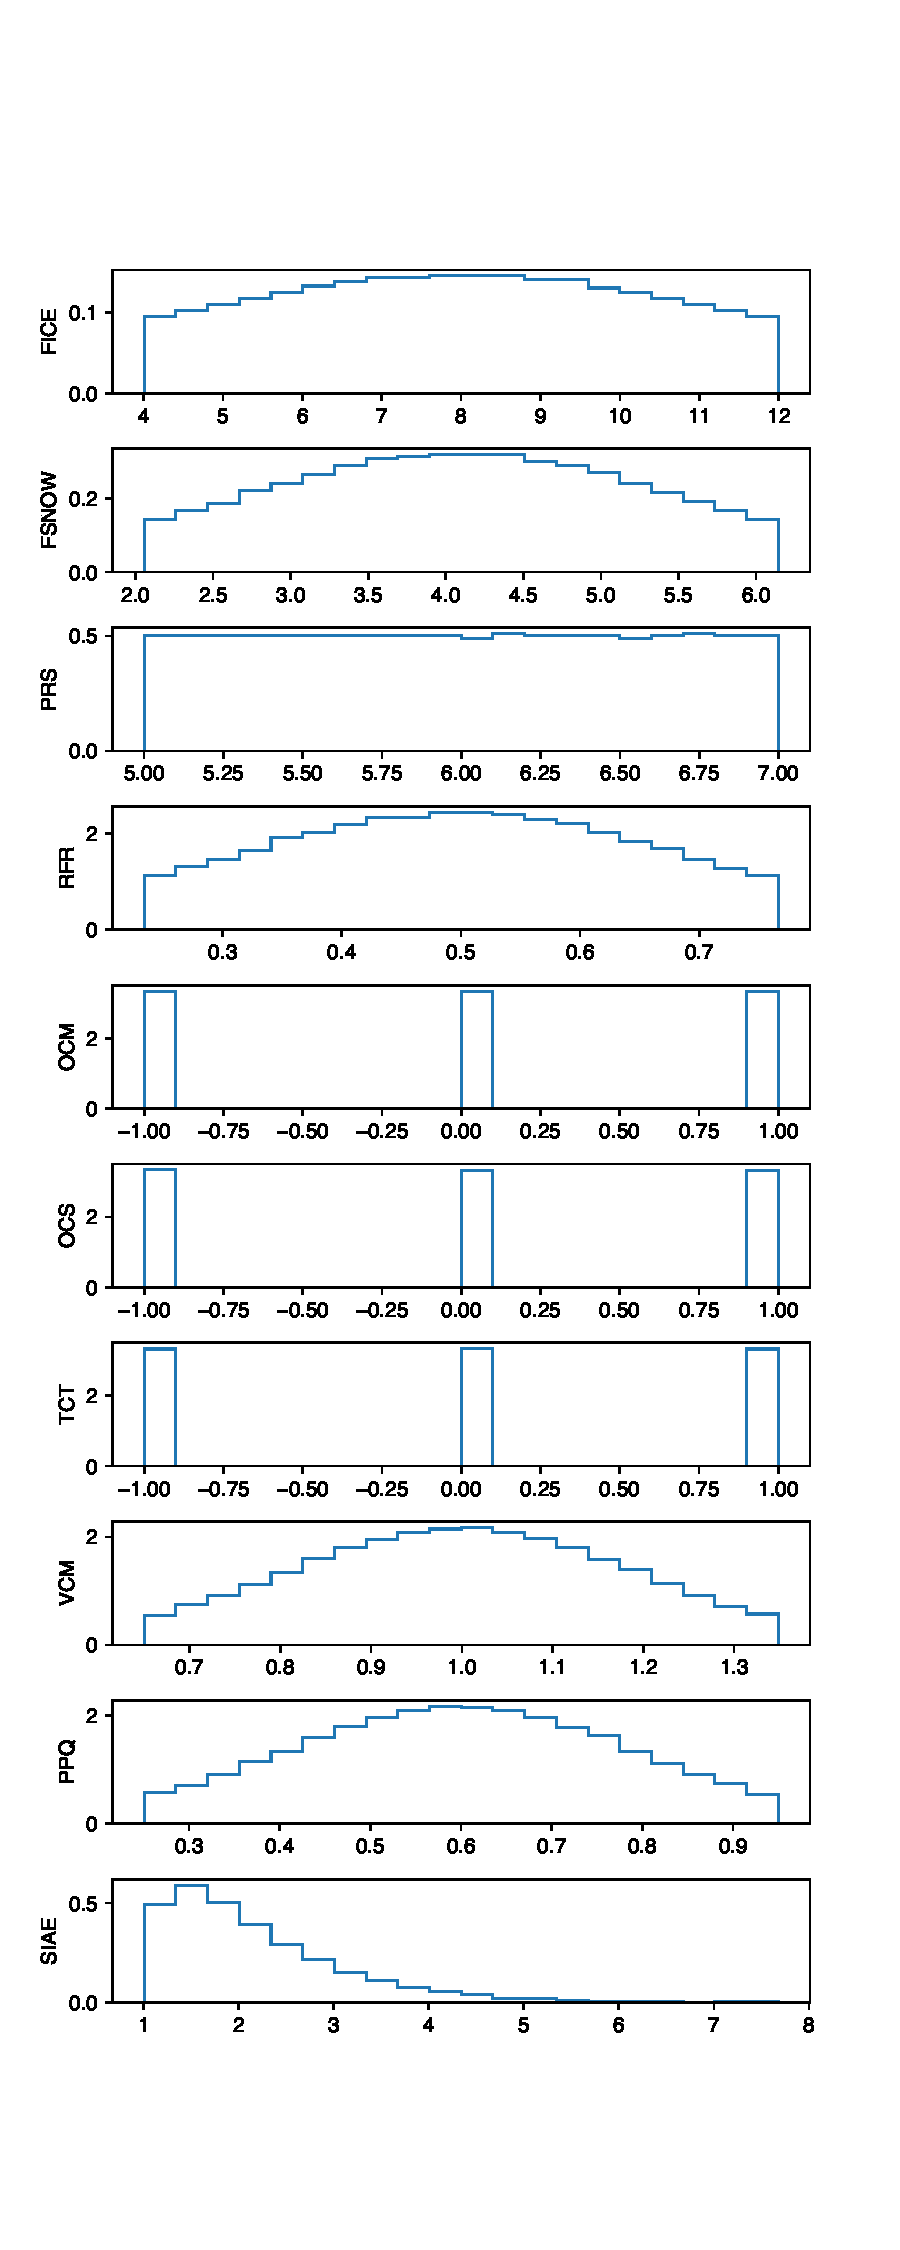
\includegraphics[height=8.5cm]{lhs_histograms}
      \end{figure}
    \end{column}
    \begin{column}{.6\linewidth}
      \begin{itemize}
      \item for each RCP scenario, draw 500 samples from distributions
      \item 1,500 Large Ensemble Simulation
      \item calculate Sobol indices to attribute uncertainties to parameters
      \end{itemize}
    \end{column}
  \end{columns}
\end{frame}


\begin{frame}
  \frametitle{Temperature anomalies}
  \begin{figure}
    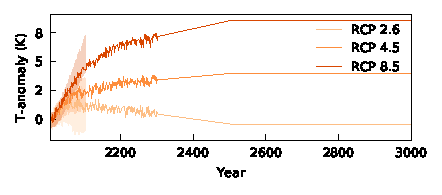
\includegraphics[width=\textwidth]{giss_cmip5_delta_T}
    \caption{Temperature anomalies with respect to 2006--15 derived from NASA GISS ModelE-2 simulations that extend until 2300. Beyond 2300, the linear 2200--2300 trend was extrapolated to 2500, after which the 2500 value was kept constant. The shaded area indicates $\pm1\sigma$ of the CMIP5 multi-model ensemble.}
  \end{figure}
\end{frame}


\begin{frame}
  \frametitle{Temperature and precipitation}
  \begin{figure}
    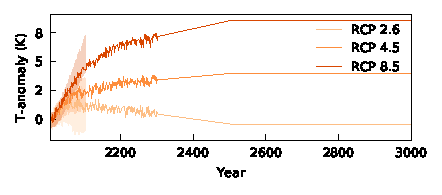
\includegraphics[width=\textwidth]{giss_cmip5_delta_T}
    \caption{Temperature anomalies with respect to 2006--15 derived from NASA GISS ModelE-2 simulations that extend until 2300. Beyond 2300, the linear 2200--2300 trend was extrapolated to 2500, after which the 2500 value was kept constant. The shaded area indicates $\pm1\sigma$ of the CMIP5 multi-model ensemble.}
  \end{figure}
\end{frame}

\begin{frame}
  \frametitle{Ocean melt rates}
    \begin{columns}[c]
    \begin{column}{.4\linewidth}
      \begin{figure}
        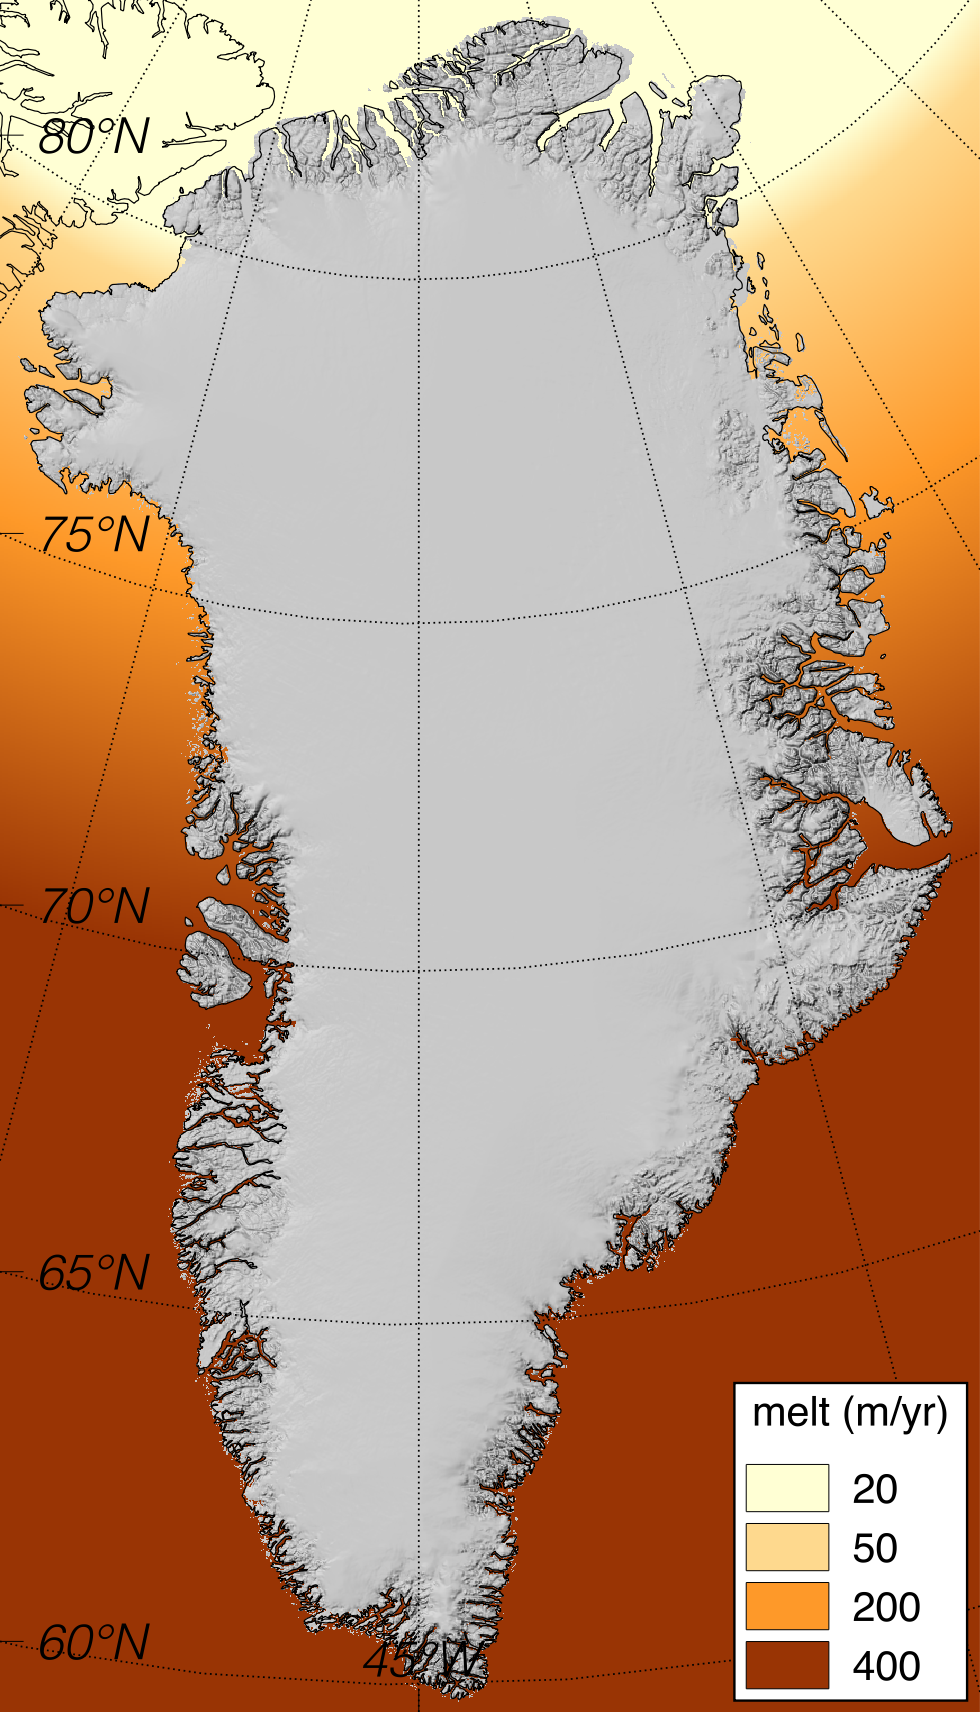
\includegraphics[height=7.5cm]{ocean-forcing}
      \end{figure}
    \end{column}
    \begin{column}{.6\linewidth}
      \begin{itemize}
        \item latitudinal dependence
      \end{itemize}
    \end{column}
  \end{columns}
\end{frame}


\begin{frame}
  \frametitle{Ocean melt rate anomalies}
  \begin{figure}
    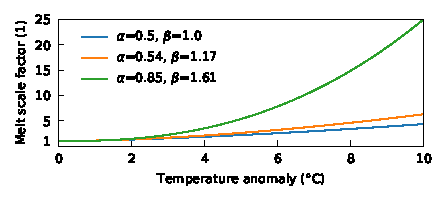
\includegraphics[height=5cm]{temp2melt}
  \end{figure}
\end{frame}

\begin{frame}
  \frametitle{The next thousand years}
  \begin{figure}
   \movie[showcontrols=true,autostart,loop,width=12cm]{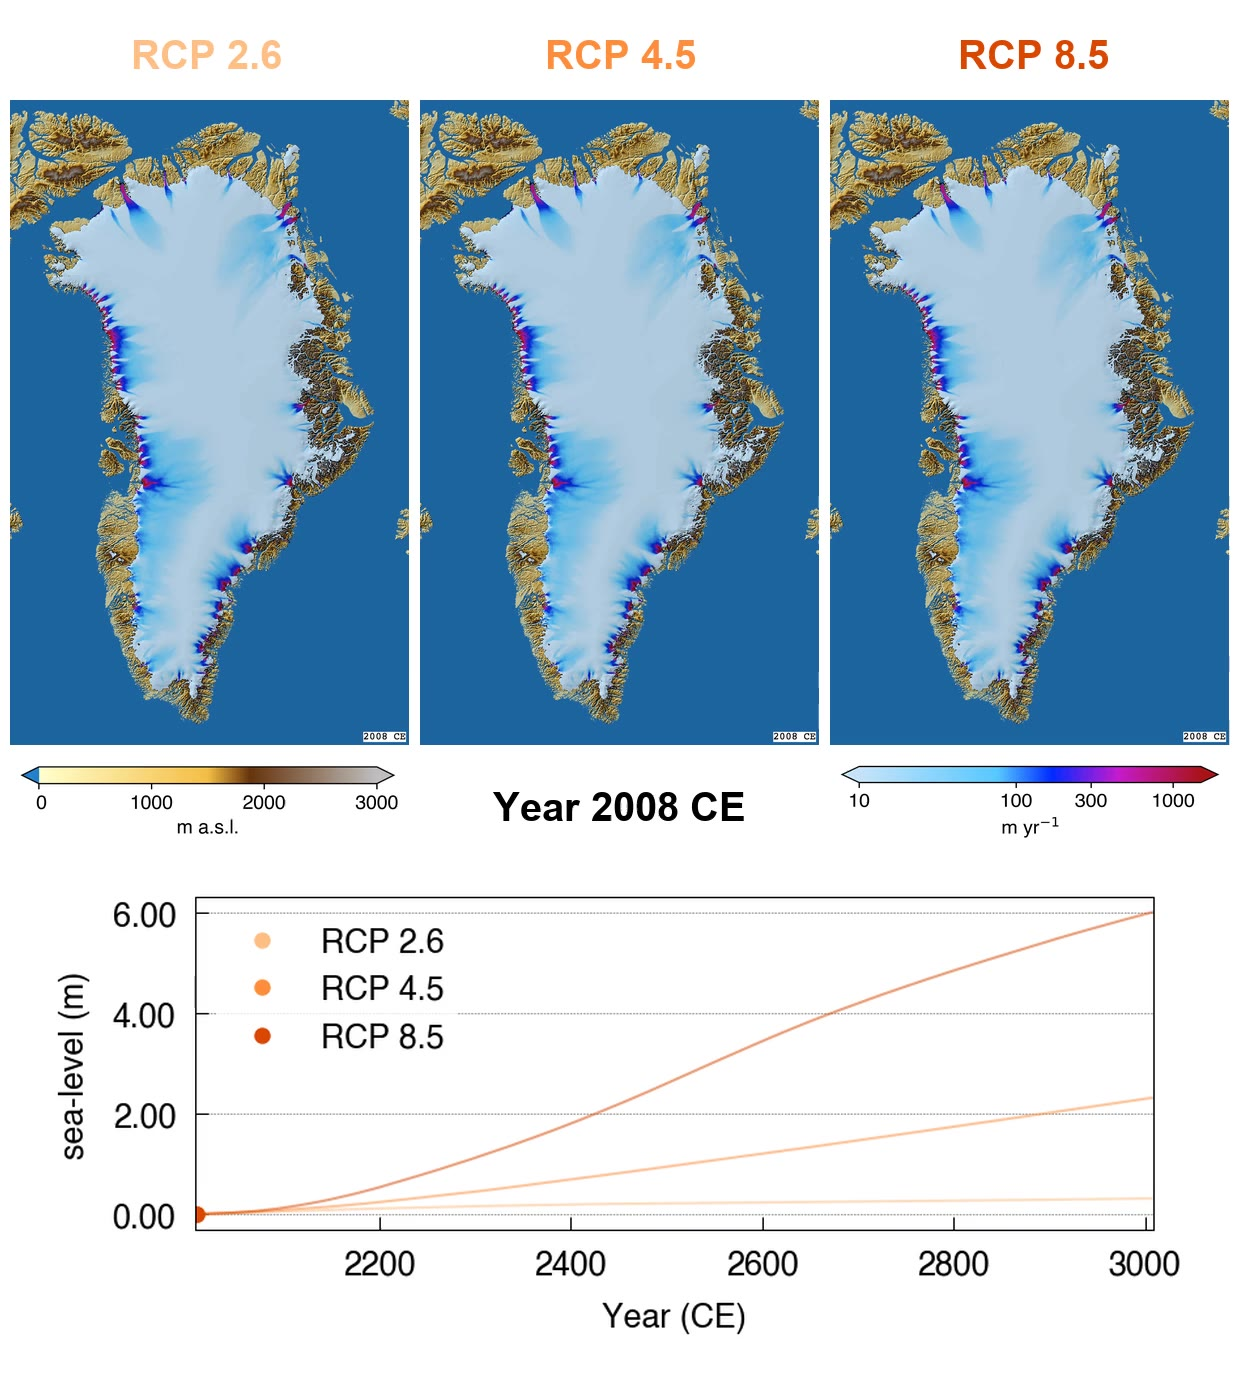
\includegraphics[width=12cm]{../movies/gris-g1200m_rcps-hd1920}}{../movies/gris-g1200m_rcps-hd1920.mov}
  \end{figure}
\end{frame}


\begin{frame}
  \frametitle{Evolution over the next millennium}
  \begin{figure}
    \includegraphics<1>[height=5cm]{les18_rcp_limnsw}
    \includegraphics<2>[height=5cm]{les18_rcp_tendency_of_ice_mass_glacierized}
  \end{figure}
\end{frame}

\begin{frame}
  \frametitle{Outlet glacier retreat}
  \begin{figure}
    \includegraphics<1>[height=7.25cm]{rcp45_Upernavik_Isstrom_S}
    \includegraphics<2>[height=7.25cm]{rcp45_Store_Gletscher}
  \end{figure}
  \vspace{-0.5cm}
  \begin{figure}
    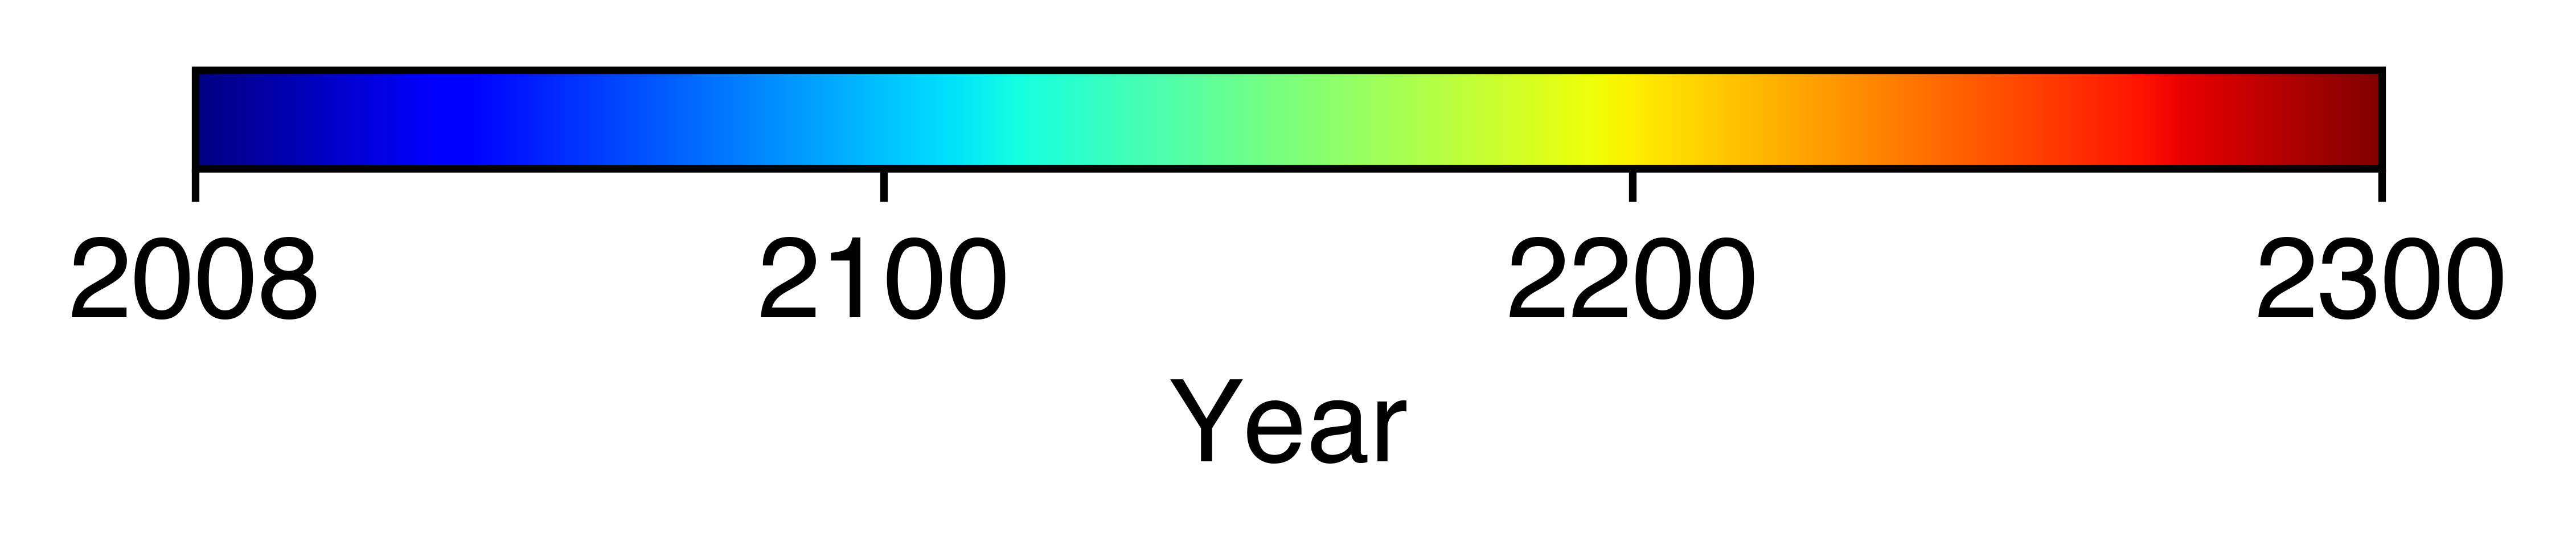
\includegraphics[height=1cm]{jet_horizontal}
  \end{figure}
\end{frame}


\end{document}